\chapter{Discussion}
\label{chapter:discussion}
% from master thesis contract: Discuss how a well-performing representation learning model on protein sequences can be used for exploring new proteins and their properties, and other potential applications, if any.

% The major findings of your study
% The meaning of those findings
% How these findings relate to what others have done
% Limitations of your findings
% An explanation for any surprising, unexpected, or inconclusive results
% Suggestions for further research

In this chapter we will discuss the results from chapter \ref{chapter:experiments} as a whole, comparing the models to each other. In section \ref{sec:comparison_representations}, we compare the representations and the results that the models achieved in the experiments. We also discuss what may cause the differences in performance between the models and suggest alternative ways to extract the representation from UniRep or WaveNet. In section \ref{discussion:data}, we discuss the role that the data may have in the good performance of the VAE, as well as the limits that the data imposes onto the significance of our experiments. In section \ref{sec:protein_exploration}, we discuss how the latent space of representations may be used for exploration in the protein space and how this may require additional tinkering. Finally, in section \ref{sec:further_work}, we consider avenues for further work that build on the ideas that we have worked on.

%  discuss the trade-offs between the latent spaces of different models

% {discuss why learning rate is immensely important; shifting the lr a little bit basically means the models learn almost nothing} 

\section{Comparison of Experimental Representations}
\label{sec:comparison_representations}
Based on experimental results alone, there are some clear guidelines to which models produce the most ideal protein representations. For convenience, figure \ref{fig:MEP_barchart} and \ref{fig:TAPE_barchart} compare models across the two experimental settings.

% \label{discussion:representations}
\begin{figure}[H]
    \centering
    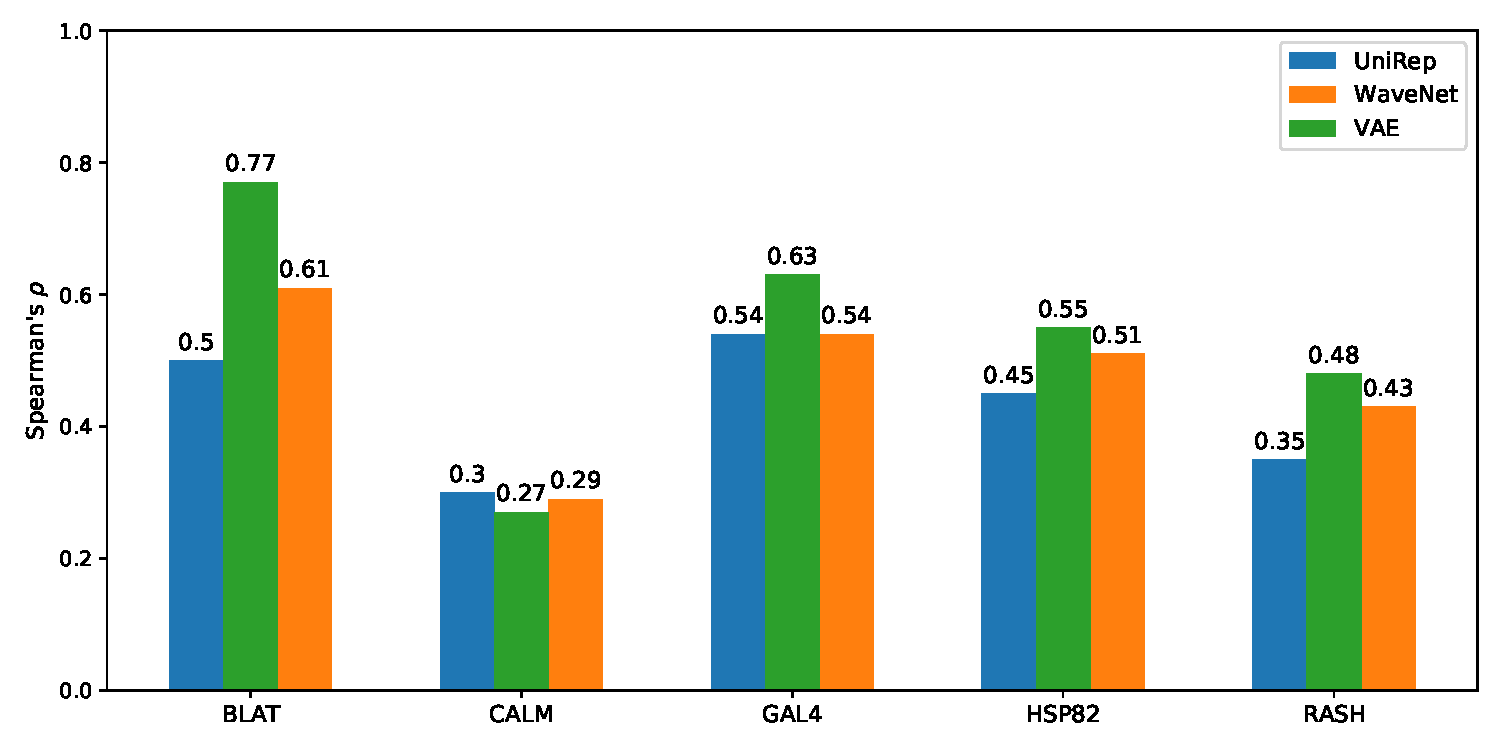
\includegraphics[width = 0.9\linewidth]{report/figures/MEP_barchart.pdf}
    \caption{Bar chart comparing each of the three model variants on the five protein families tested. The generally best configurations for each model are shown. Almost invariably, VAE is best with WaveNet at second place. The exception is CALM, but even then the difference is hardly significant.}
    \label{fig:MEP_barchart}
\end{figure}

\begin{figure}[H]
    \centering
    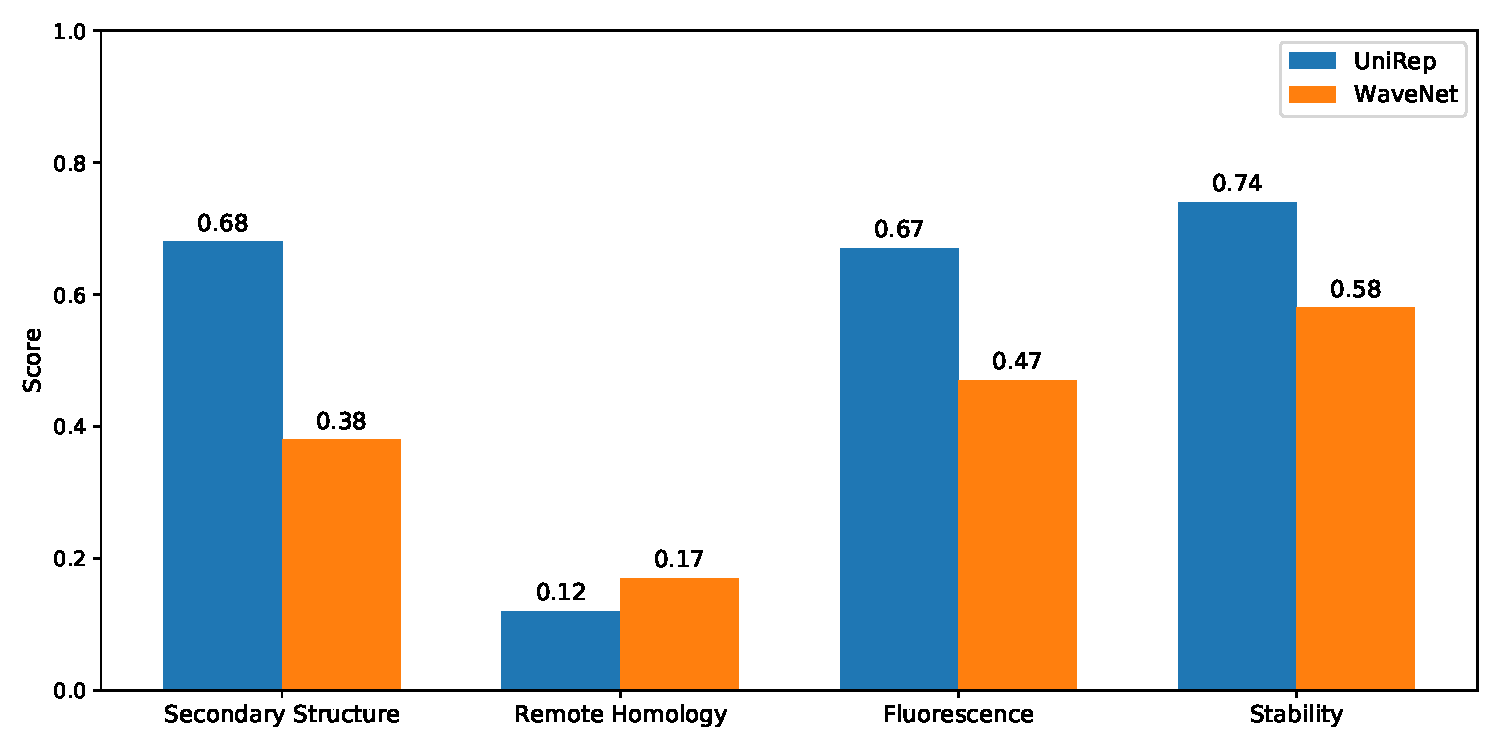
\includegraphics[width=0.9\linewidth]{report/figures/TAPE_barchart.pdf}
    \caption{Bar chart comparing UniRep and WaveNet on the TAPE tasks. The generally best configurations for each model are shown. UniRep outperforms WaveNet on all but the remote homology task.}
    \label{fig:TAPE_barchart}
\end{figure}

For family-specific, local representations, the VAE outperforms both the WaveNet and UniRep across the five protein families tested. There are several reasons why this might be the case.

One reason is that the aligned protein sequences is a strong signal to the model that is not preserved otherwise. However, the performance of WaveNet and UniRep on $\beta$-lactamase with sample weights, taken from the aligned dataset, suggests that it is not the alignment itself that is important. That is, the significant performance increase is not from the insertion of gaps, but rather from the similarity measure and reweighing of samples according to their uniqueness, that such an alignment affords. Data- and preprocessing related aspects are discussed in section \ref{discussion:data}.

Another reason might be the fact that the representation is explicitly trained by the model, allowing for the model to fully decide, within its capacity, what should be retained and what should be discarded in the representation. 

In addition, the underlying probabilistic setting is different for the VAE. Specifically, when making predictions, the model can consider all positions indirectly through the latent space representation. In contrast, UniRep and WaveNet are constrained to the positions observed so far. This is somewhat mitigated by the bidirectional ensemble of the WaveNet, and a similar extension can be made to UniRep, but it still raises the practical issue of concatenating a ``forward''-- and a ``backward'' representation of the same protein in such cases. The VAE setting has no such issues.

Finally, the space of the representations itself affords several advantages in exploratory protein settings, as discussed further in section \ref{sec:protein_exploration}.

While latent spaced representations have some favorable advantages in comparison with the representations of UniRep and WaveNet, the major downside is that they cannot directly be applied to a broader, more general set of proteins. If the desired protein representation is to be broadly applicable, our experiments suggest that this will likely compromise the performance on local subsets of proteins. WaveNet's relatively good results on mutation effect prediction and comparatively bad results on TAPE, and vice versa with UniRep may suggest that there is a trade-off in a model's capacity in the local and global protein scale. It seems clear at least that, if one is constrained to work with unaligned proteins, UniRep is to be favoured in the global scale while WaveNet is favoured on the local scale. WaveNet is at a huge disadvantage on all tasks but stability on TAPE, whereas UniRep is only marginally worse than WaveNet on mutation effect prediction. This might indicate that the WaveNet architecture is fundamentally worse at producing representations that work well across diverse tasks, whereas UniRep seems to be able to handle both diverse, general tasks and local finetuning. It does not seem impossible that UniRep can perform comparably to WaveNet on mutation effect prediction if properly augmented, whereas it might require serious rethinking of WaveNet to yield comparable results to UniRep on TAPE.

\subsection{Extracting Representations}
\label{sec:extracting_representations}
The representations that our models produce are quite different. The VAE inherently includes a bottle-necked representation, which allows the representation to become part of the training procedure. The UniRep and WaveNet models do not have this luxury, as the representations must be extracted after training. The task of extracting a suitable representation from models that take variable length sequence inputs is nontrivial. In our settings, we have applied the naive approach of collapsing the position-wise representations (i.e. the hidden state for UniRep and residual channels for WaveNet) in the models by taking the mean. This has the positive effect of being effective and simple, but it also has significant downsides. Specifically, such an operation is hard to reverse, and as a consequence a protein sequence cannot easily be recovered from its representation. In terms of protein exploration this is critical, as the representation space cannot be explored in search of new proteins, as you would not be able to recover a protein sequence from a representation of interest.

A mean representation does not preserve any position-related properties of the protein. Any feature that denotes local characteristics of the protein is made less relevant by the mean across the entire sequence. Imagine a single feature dimension that encodes if the current position is part of an $\alpha$-helix or not. The mean of such a dimension would override such information, yielding instead the $\alpha$-helix proportion of the entire protein sequence. In this sense, the mean is a crude operation with no explicit mechanism to retain such important information present in the position-encoded representations.

On the other hand, fixed-length representations of proteins with variable length inevitably need to be position-agnostic, as should be encouraged if fundamental protein properties are to be captured. Ideally, a suitable representation should be learned explicitly during model training, as in the VAE architecture, making manually engineered extraction schemes superfluous. A line of work that should at least be explored is to combine the built-in representation of the autoencoder with the variable-length models, as sketched in figure \ref{fig:sketch}. A major problem with this approach is that the decoder model has to reconstruct a variable length-sequence from a fixed representation, which is a daunting task. It can be mitigated by teacher-forcing or by producing a beam search instead of a single prediction path, but only the latter will be viable outside training settings. Such a model would be able to explicitly train on the task of autoencoding arbitrary-length proteins into fixed-size representations. 
\begin{figure}[H]
    \centering
    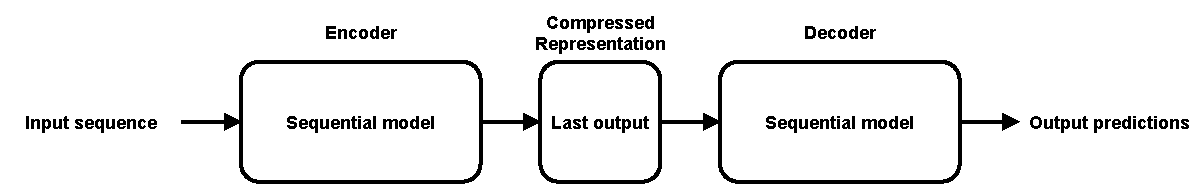
\includegraphics[width = \linewidth]{report/figures/sketch.pdf}
    \caption{A sketch of an autoencoding model that produces fixed-length representations over variable-length sequence input. The input is passed through an encoding architecture that is able to process sequential inputs, such as the LSTM (like UniRep) or a convolution-based model (like WaveNet). The last output of the encoder could function as the compressed representation of the input, as this is explicitly trained by the model, making the architecture itself figure out what should be retained. Then, a similar architecture functions as a decoder whose task it is to reconstruct the input from the representation.}
    \label{fig:sketch}
\end{figure}

Models like the one sketched in figure \ref{fig:sketch} have been created before within natural language processing, but we have yet to see this method be truly effective in protein machine learning, especially on arbitrary, non-aligned proteins. Other things being equal, explicitly training the network to construct representations should be preferred to manual engineering. 

% specifically, we discussed the choice of making a representation of a protein sequence that is constituted by the average of the hidden states at each position in the sequences. This choice does not preserve any position-related features of the protein, nor does it easily allow for a reversible procedure, regaining the sequence from its representation. Finally, it complicates the interpretation of the representation: units that give a clear signal to some property of the protein in local positions potentially loose relevancy when averaged. These arguments suggest that even though the representation capture fundamental protein features that performs well in downstream tasks, the design of the representation is problematic for other tasks, e.g.  tasks that require a feature space where the representation can be reversed

% discuss why alignments are so powerful/important for the results

\section{Data and preprocessing}
\label{discussion:data}
Our findings show that the VAE is generally superior on the mutation effect prediction task, when compared to the other models. However, it is worth noting that the VAE does not only have the advantage of an explicit trained encoder-representation-decoder network, but also the advantage of a fixed-size protein alignment as data. As discussed previously in section \ref{sec:sequence_alignments}, sequence alignments can be made in many different ways, consequentially with varying performance on downstream tasks. This is also true for the VAE model. The question is, how much of the VAEs better performance, in comparison to the competition, comes from the architecture versus the preprocessing of the data through an alignment? Ideally, we'd like to be able to attribute the performance of the VAE to its architecture, but this does not seem to be the entire influence. As evidenced by WaveNet's improved performance when given weights based on an alignment, preprocessing of the data into a neater structure can significantly improve performance. This suggests that a significant portion of the VAE's greater performance comes from the preprocessing of the proteins into an alignment, rather than the VAE's own architecture. %A model which could achieve the same performance while not requiring an alignment would be truly impressive, but this seems to be out of reach by state-of-the-art methods at this time.

There is also a potential issue about the experimental data that we compare our predictions with. Each protein family in the mutation effect prediction task uses a separate set of experimental data to calculate the correlation coefficients. However, this correlation coefficient is oblivious about the other experimental data gathered on the mutations and thus the whole effect of the mutation on the protein cannot be determined by our models alone. This problem is also brought up by \textcite{riesselman2018deep}, where they note that a ``mutation may be damaging with regard to some measurable protein feature -- for example, enzyme efficiency -- but harmless for stability or even organism fitness''. That is, we need to remember that our results only highlight the correlation with one specific experimental data measure and we have no data on our models' performances on other experimental measures.

% One surprising result seems to be that pretraining on global protein space, i.e. the UniRef50 protein sequence dataset, causes a drop in performance. The data generating process might explain why we see this happening. Unlike our protein family datasets, UniRef50 is not cut in the ends, and protein sequences are in general longer in that dataset. UniRef50 is a boiled down version of UniRef100, heuristically clustered, whereas the protein family datasets are obtained using Hidden Markov Models.

% \{discuss alignment-related problems, i.e. this is a huge influence and the ``ad-hoc'' cutting and slicing of protein alignments for each family is not very general. In fact, how much of the performace we observe is caused by the preprocessing? We would like to at least be able to attribute performance to the model itself and not differences in how the datasets are preprocessed. Ideally, the model should take raw sequences with no cutoffs and be performant under those settings.}

% \{discuss this exerpt from \cite{riesselman2018deep}: ``the premise that evolutionary data can be applied to predict outcomes of an experiment is highly contingent on the relevance of the experimental assay to long-term selective forces in the family. A mutation may be damaging with regard to some measurable protein feature e.g. enzyme efficiency, but harmless for stability or even organism fitness''}

\section{Protein Exploration}
\label{sec:protein_exploration}
Figure \ref{fig:2dimvae} shows an interesting result about the landscape of the VAE's protein representations. Figure \ref{fig:unirep_tsne} shows a similar picture, although one must remember that this is from a non-linear transformation of the data and hence not directly comparable to the points' distribution in 512 dimensions. These figures suggest that the protein representation landscape resembles a phylogenetic tree at a high level. The zoomed-in view in figure \ref{fig:2dimvae} suggests that the landscape is (at least locally) smooth -- that is, small changes in the protein lead to small changes in the representation. This is an especially important property when one's goal is to explore the representation space (and by extension, the space of proteins).

However, it does not seem like the smoothness of the representation space at the small scale translates into a regular euclidean distance measure at larger scales. There are large areas between the phylum clusters where there are no representations provided by the data -- in principle, these empty areas contain representations just like the phylum clusters do, but the question is whether these representations are meaningful, when it is clear that the data has not informed these areas. For example, one way to explore the representation space may be to interpolate between two proteins that inhabit separate phylum clusters in the representation space. A naive linear interpolation would likely not be effective, as this would frequently cross areas where the data is not present and thus likely to be noisy or otherwise meaningless. Such a linear interpolation is shown in figure \ref{fig:interpolation}.

An effective exploration of the protein representation space might require a non-euclidean distance measure, which takes into account the phylogenetic tree-like structure. An interpolation between two protein representations using such a distance measure may be able to interpolate along data-populated areas, rather than traversing empty, high-uncertainty areas.

% \{This is one of our learning objectives from the thesis contract: Discuss how a well-performing representation learning model on protein sequences can be used for exploring new proteins and their properties, and other potential applications, if any}

\begin{figure}
    \begin{center}
    \begin{tabular}{c}
    \begin{lstlisting}[basicstyle=\ttfamily\footnotesize]
...LKAQIQELAAKYKLTPGVFFVDLDTGAYV.DINGDTPFPAASTIKLPILIAFFQDVDAGKIRLDEKLTMTEELIGGG
...LKAKIQALAAQYKLTPGVFFVDLDTGAYV.DINGDTPFPAASTIKLPILIAFFQDVDAGKIRLDEKLTMTEEDIGGG
...LKAKIQALAAQYKLTPGVFFVDLDTGAYV.DINGDTPFPAASTIKLPILVAFFQAVDAGKISLDEKLTMTEEDIGGG
...LK.KIQALAAQYGLTPGVFFVDLDTGAYV.DINGDTPFPAASTIKLPILVAFFQAVDAGKISLDEKLTLTEEDIVGG
.......I..L.A.YGLTPGVALVDLDTGEYL.DINGDEPFPAASTIKLPILVAFFQAVDAGKISLDEKLTLTEEDIVGG
..........L....DL.V..FLADLDDGRYL.ELNADEPFPAASTIKLPILVAFFEAVDAGKISWDEPLTLTEDVIGGG
..........L...KDL.V..FVADLDDGRYL.ELNADEPFPAASTIKLPILLALFEAVDQGKISWDEPLELTEDVIGGG
.......I..L...KD.KV..YLADLDDGPVL.ELNADEPFPAASTIKLPLLLALFRAVDQG.LDWDEPLPLTNDVIVPG
.......L..L..A.P.KVS.YLARLDDGPVL.ERRADEPHNAASTIKLAVLAALFRAVDAG.LDWDEPLPVTNEFVVAG
..........LLAA.PGTVSVYLGRLGGGPSF.SRRADRPHYAASTIKLAVLAALFRAVEAGELDLDEPVPVTNEFVVAG
............AA.P.TISIYLGRLGGGPSF.SRDADRPHYAASTIKLAVLAAVFRAVD.GELDLDEPVPVRNEFRVAG
.............A.P.TVSVAAADLDGGPVL.SRDADRPFYAASTMKLALLAAVARAVD.GELDLDEPVPVRPEFRVAG
.............A...TWSV.VVDLDGGEVL.SHDADRVLPTASVGKLLLLAAVARRLDAGELDPDEPLELRPDDRVGD
...................S..I.DLDGGEVL.E.NADEVLPAASVGKLFLLAAVARAVD.GELDLDERVTLTAEDRVPD
..........................N.G........DER...ASTGK.FLAAAVL.A.T.GELDLDQKVTITAEDLVPH
.......L.EL.KKYG.KIGVYILDTENGKII.SHN.DERFPYASTYKALAAGVLLEKLT..PDDLNKKIPIKKSDLVTY
...LQKELAELEKKYGGKIGVYALNTENGKQI.SYNADERFPIASTYKVLAAGALLKKSPQGPDLLNQKIPYKKSDLVSY
...LEQKLAALEKDFGGRLGVYAIDTANGKQI.SYRADERFPMASTFKVLAAAALLKKSQKDPALLDQKIRYTKSDLVSY
...LEAQLAALEKSAGGRLGAAAIDTANGRQI.SYRADERFPLCSTSKVMAAAAILKKSQTDEGLLDKRIHYSKADLVEY
.....AQLAALERSFGGRLGVAALDTGSGRTV.GYRADERFPFCSTFKAMLAAALLKRSPQDEGLLDQRIHYTKADLVEY
.....ARLAALERRFGGRLGVFALDTGSGRTV.AHRADERFPFCSTFKALLAAAVLRRAPQDPGLLDQRIHYTKADLVEY
.....ARLAALERRFGARLGVYALDTGSGRTV.AHRADERFAFCSTFKALAAAAVLRRAPQGEGLLDQRIHYTPADLVPY
......RLAELERRFNARIGVYALDTGTGRTV.AHRADERFAMCSTFKAYAAAAVLQRAQQGELSLDQRVHYDPADIVPN
......RLAELERRYNARIGVYAVDLGGGRTV.AHRADERFAMCSTFKAYAAAAVLQRAQRGELSLDQRVHIDPADIVPN
.....ARLAELERRYNARIGVFAVDLDGGRTV.AHRADEPFAMCSTFKAYAAAAVLQRYQRGGLSLDQRVHIDPADIVPN
\end{lstlisting}
\end{tabular}
\end{center}

    \caption{Naive linear interpolation in the two-dimensional latent space (shown in figure \ref{fig:2dimvae}) between two protein representations in the $\beta$-lactamase protein family results in the above proteins once decoded. Only the first 80 positions of the alignment are shown. The 25 representations are evenly spaced. A dot (``\texttt{.}'') indicates a gap in the aligned sequence.}
    \label{fig:interpolation}
\end{figure}

% \section{Representation Applications}

% Noget Daniele har sagt: it will be useful to use representation to explain the behavior of variants of protein that we know, but we need to optimize. For example, the representation is important to help explaining the experimental results of variants screening, trying to map the effect of mutations, especially in case when we don’t have a structure.
